\section{Appendix}

\subsection{Table with the used hyperparameters that deviate from Scikit-learn's default settings}
\label{ssec:ushp}
\begin{table}[h]
\begin{footnotesize}
\begin{tabular}{lll}
    \toprule
    \textbf{Algorithm}                  & \textbf{Scikit-learn}     & \textbf{Hyperparameters}  \\
    \midrule
    Nearest Neighbors                   & NearestNeighbors()        & n\_neighbors = 2          \\
                                        &                           & algorithm = “brute”       \\
    \midrule
    K-Nearest Neighbors                 & KNeighborsClassifier()    & n\_neighbors = 8          \\
    \midrule
    RandomForest                        & RandomForest()            & n\_estimators = 231       \\
                                        &                           & min\_samples\_split = 2   \\
                                        &                           & min\_samples\_leaf = 1    \\
                                        &                           & max\_features = “sqrt”    \\
                                        &                           & max\_depth = None         \\
                                        &                           & bootstrap = False         \\
                                        &                           & random\_state = 7         \\
    \midrule
    Logistic Regression                 & LogisticRegression()      & random\_state = 0         \\
                                        &                           & solver = “sag”            \\
                                        &                           & multi\_class = “ovr”      \\
                                        &                           & max\_iter = 10000         \\
    \midrule
    Linear Support Vector Classification& LinearSVC()               & random\_state = 7         \\
    \midrule
    Neural Network                      & MLPClassifier()           & activation = ‘relu’       \\
                                        &                           & hidden\_layers\_sizes = dataset length    \\
                                        &                           & learning\_rate = “constant”   \\
                                        &                           & max\_iter = 10000         \\
                                        &                           & n\_iter\_no\_change = 10  \\
                                        &                           & random\_state = 7         \\
                                        &                           & solver = “adam”           \\
                                        &                           & early\_stopping = “False” \\
    \bottomrule
\end{tabular}



\end{footnotesize}
\caption{\label{tab:Hyperparameters} The used hyperparameters that deviate from Scikit-learn's default settings}
\end{table}

\subsection{Two graphs that picture the search of the optimum number of neighbors for K-Nearest Neighbors}
\label{ssec:fonn}
\begin{figure}[h]
    \centering
    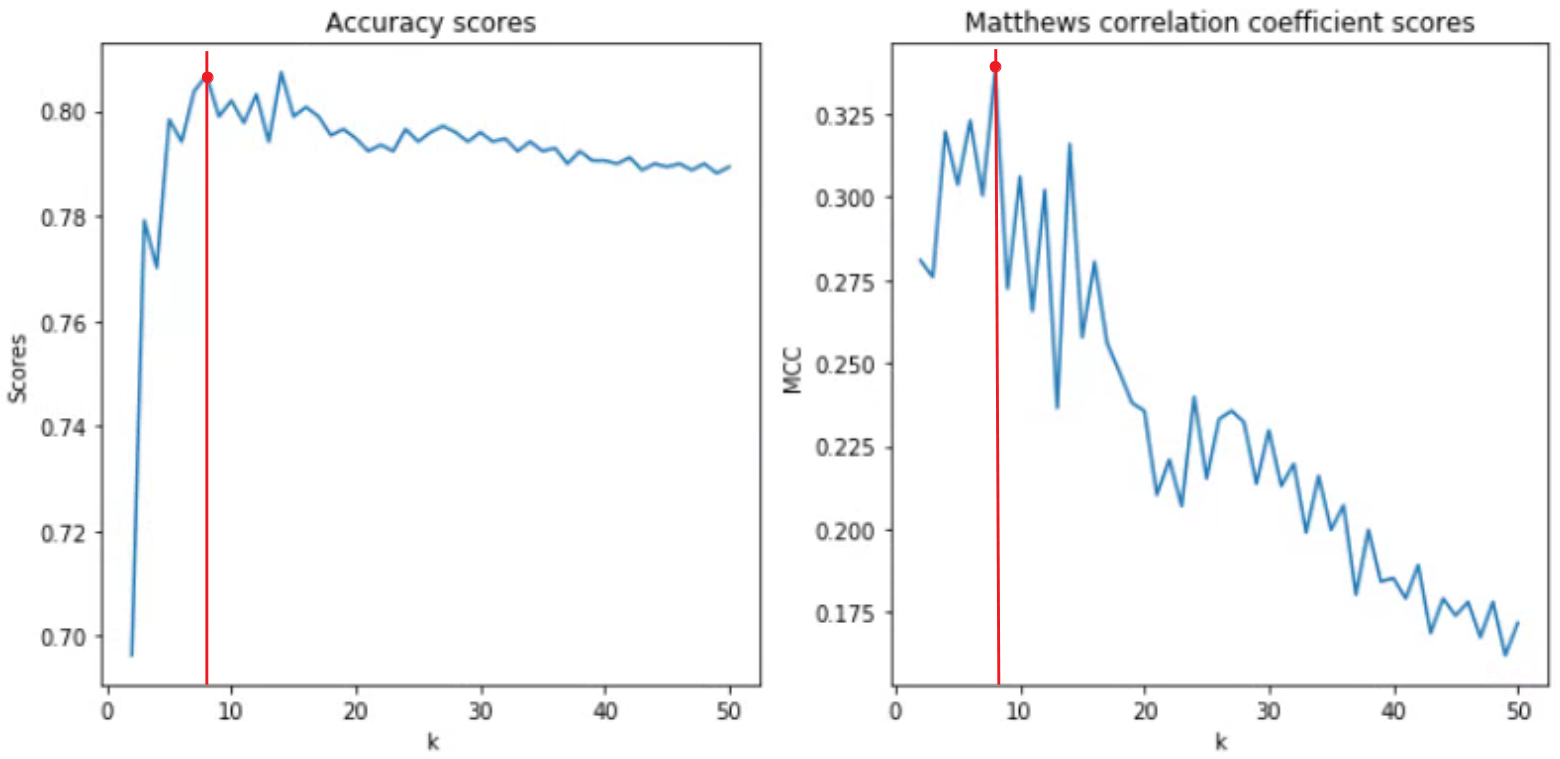
\includegraphics[width=.7\linewidth]{ThesisTemplate/Images/KNN_n_neighbors.png}
    \caption{Determining of the optimum number of neighbors for K-Nearest Neighbors}
\end{figure}

\subsection{Table with the scenarios and the results of K-Modes clustering for the Neural Network}
\label{ssec:cluscen}
\begin{table}[H]
\begin{footnotesize}
\begin{tabular}{llllll}
\toprule
\textbf{Scenario}   & \textbf{Features (\textit{X})}    & \textbf{Labels (\textit{y})}  & \textbf{Clusters} & \textbf{Accuracy} & \textbf{MCC}        \\
\midrule
baseline            & users + jobs                      & labels                        & -                     & 0.81              & 0.44            \\
baseline            & users                             & labels                        & -                     & 0.71              & 0.03            \\
baseline            & jobs                              & labels                        & -                     & 0.84              & 0.53            \\
\midrule
1                   & users + jobs + user clusters      & labels                        & 225                   & 0.81              & 0.41            \\ %6.7
2                   & jobs + user clusters              & labels                        & 275                   & 0.82              & 0.49            \\ %6.15
3                   & users + user clusters             & labels                        & 300                   & 0.75              & 0.08            \\ %6.8
4                   & user clusters                     & labels                        & 100                   & 0.77              & 0.05            \\ %6.13
5                   & users + jobs + job clusters       & labels                        & 225                   & 0.82              & 0.45            \\ %6.2
6                   & users + job clusters              & labels                        & 300                   & 0.77              & 0.27            \\ %6.3
7                   & jobs + job clusters               & labels                        & 250                   & 0.84              & 0.55            \\ %6.14
8                   & job clusters                      & labels                        & 150                   & 0.79              & 0.27            \\ %6.12
9                   & users                             & job clusters                  & 25                    & 0.15              & 0.11            \\ %6.4
10                  & users + jobs                      & job clusters                  & 25                    & 0.93              & 0.92*            \\ %6.6
12                  & jobs                              & user clusters                 & 25                    & 0.11              & 0.05            \\ %6.10 
13                  & users + jobs                      & user clusters                 & 25                    & 0.89              & 0.88*            \\ %6.11
\bottomrule
\tiny{*Overfitting} \\
\end{tabular}

\end{footnotesize}
\caption{\label{tab:clusc} K-Modes clustering scenarios \& results for the Neural Network}
\end{table}

\subsection{Elbow plot showing the search of the optimum number of clusters for the K-Means clustering of the top 1000 TF-IDF scores of the job descriptions}
\label{ssec:Kmeans}
\begin{figure}[h]
    \centering
    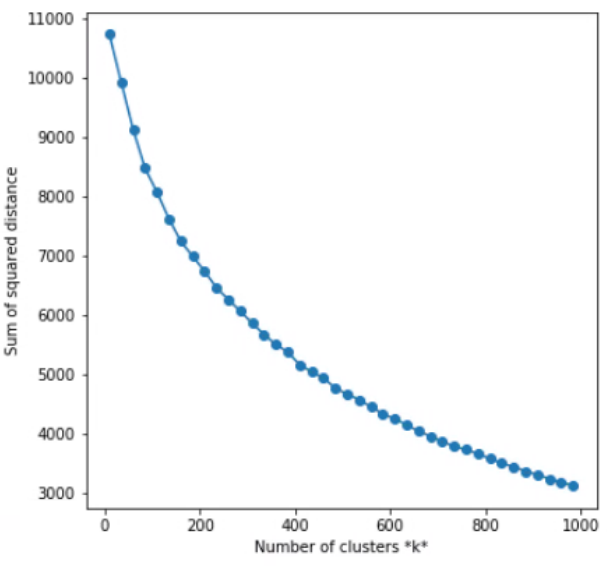
\includegraphics[width=.4\linewidth]{ThesisTemplate/Images/K-means.png}
    \caption{Elbow plot of the clustering of TF-IDF scores with K-Means}
\end{figure}

\subsection{Table with the Hierarchical Clustering scenarios and results of the clustering if n-grams of characters of job titles for the Neural Network}
\label{ssec:hieclu}
\begin{table}[H]
\begin{footnotesize}
\begin{tabular}{lllll}
\toprule
\textbf{Scenario}   & \textbf{Features (\textit{X})}    & \textbf{Labels (\textit{y})}  & \textbf{Accuracy} & \textbf{MCC}        \\
\midrule
baseline            & users + jobs                      & labels                        & 0.81              & 0.44            \\
baseline            & jobs                              & labels                        & 0.84              & 0.53            \\
\midrule
1                   & users + jobs + job clusters       & labels                        & 0.81              & 0.41            \\ %6.2
2                   & users + job clusters              & labels                        & 0.74              & 0.10            \\ %6.3
3                   & jobs + job clusters               & labels                        & 0.83              & 0.48            \\ %6.14
4                   & users                             & job clusters                  & 0.25              & 0.04            \\ %6.4
5                   & users + jobs                      & job clusters                  & 0.71              & 0.66            \\ %6.6
\bottomrule
\end{tabular}

\end{footnotesize}
\caption{\label{tab:hieclu} Hierarchical Clustering scenarios and results for the Neural Network}
\end{table}

\subsection{Table with the classification results for all models}
\label{ssec:cm}
\begin{table}[H]
\begin{footnotesize}
\begin{tabular}{llrr}
    \toprule
    \textbf{Algorithm}                  &                           &                           &                           \\
    \midrule
    Nearest Neighbors                   &                           & Positive Labels           & Negative Labels            \\
                                        & Positive Labels           & 5,482                     & 1,008                      \\
                                        & Negative Labels           & 982                       & 793                        \\
    \midrule
    K-Nearest Neighbors                 &                           & Positive Labels           & Negative Labels            \\
                                        & Positive Labels           & 1,184                     & 56                         \\
                                        & Negative Labels           & 259                       & 112                        \\
    \midrule
    RandomForest                        &                           & Positive Labels           & Negative Labels            \\
                                        & Positive Labels           & 1,203                     & 37                         \\
                                        & Negative Labels           & 256                       & 115                        \\
    \midrule
    Logistic Regression                 &                           & Positive Labels           & Negative Labels            \\
                                        & Positive Labels           & 1,155                     & 85                         \\
                                        & Negative Labels           & 241                       & 130                        \\
    \midrule
    Linear Support Vector Classification&                           & Positive Labels           & Negative Labels           \\
                                        & Positive Labels           & 1,158                     & 82                        \\
                                        & Negative Labels           & 249                       & 122                       \\
    \midrule
    Neural Network                      &                           & Positive Labels           & Negative Labels           \\
                                        & Positive Labels           & 1,129                     & 111                       \\
                                        & Negative Labels           & 190                       & 181                       \\
    \midrule
    \textit{Legend}                     &                           & Positive Labels           & Negative Labels            \\
                                        & Positive Labels           & \textit{True positives}   & \textit{False negatives}   \\
                                        & Negative Labels           & \textit{False positives}  & \textit{True Negatives}    \\
    \bottomrule
\end{tabular}
\end{footnotesize}
\caption{\label{tab:cm} Classification results for all models}
\end{table}

\subsection{Table with the undersampling and oversampling results for all models}
\label{ssec:ruo}
\begin{table}[H]
\begin{footnotesize}
\begin{tabular}{l|ll|ll|ll}
& \multicolumn{2}{c|}{\textbf{Baseline}} & \multicolumn{2}{c|}{\textbf{Undersampling}}  & \multicolumn{2}{c}{\textbf{Oversampling}} \\
\toprule
\textbf{Algorithm}      & Accuracy  & MCC   & Accuracy  & MCC   & Accuracy  & MCC   \\
\midrule                       
Nearest Neighbors       & 0.76      & 0.29  & 0.69      & 0.36  & 0.78      & 0.58  \\
K-Nearest Neighbors     & 0.80      & 0.35  & 0.69      & 0.35  & 0.37      & 0.16  \\
RandomForest            & 0.82      & 0.40  & 0.78      & 0.51  & 0.80      & 0.34  \\
Logistic Regression     & 0.80      & 0.35  & 0.72      & 0.38  & 0.79      & 0.34  \\
Linear SVC              & 0.80      & 0.35  & 0.72      & 0.37  & 0.78      & 0.32  \\
Neural Network          & 0.81      & 0.44  & 0.73      & 0.40  & 0.80      & 0.39  \\
\bottomrule
\end{tabular}
\end{footnotesize}
\caption{\label{tab:ruo} Undersampling and oversampling results for all models}
\end{table}

\subsection{Table with the feature importance methods results for all models}
\label{ssec:fi}
\begin{table}[H]
\begin{footnotesize}
\begin{tabular}{l|ll|ll|ll|ll}
& \multicolumn{2}{c|}{\textbf{Baseline}} & \multicolumn{2}{c|}{\textbf{Chi-Square Test}}  & \multicolumn{2}{c|}{\textbf{BFE}} & \multicolumn{2}{c}{\textbf{RFECV}} \\
\toprule
\textit{\# Features}& \multicolumn{2}{c|}{\textit{438}} & \multicolumn{2}{c|}{\textit{180}}  & \multicolumn{2}{c|}{\textit{116}} & \multicolumn{2}{c}{\textit{115}} \\
\midrule
\textbf{Algorithm}      & Accuracy  & MCC   & Accuracy  & MCC   & Accuracy  & MCC   & Accuracy  & MCC \\
\midrule                       
Nearest Neighbors       & 0.76      & 0.29  & 0.78      & 0.33  & 0.81      & 0.46  & 0.81      & 0.46 \\
K-Nearest Neighbors     & 0.80      & 0.35  & 0.80      & 0.34  & 0.81      & 0.41  & 0.81      & 0.38 \\
RandomForest            & 0.82      & 0.40  & 0.81      & 0.37  & 0.84      & 0.50  & 0.83      & 0.50 \\
Logistic Regression     & 0.80      & 0.35  & 0.80      & 0.37  & 0.81      & 0.36  & 0.81      & 0.38 \\
Linear SVC              & 0.80      & 0.35  & 0.81      & 0.37  & 0.80      & 0.35  & 0.80      & 0.36 \\
Neural Network          & 0.81      & 0.44  & 0.80      & 0.38  & 0.81      & 0.43  & 0.83      & 0.46 \\
\bottomrule
\multicolumn{9}{l}{\tiny{BFE: Backwards Feature Elimination, RFECV: Recursive Feature Elimination with Cross-Validation}}
\end{tabular}


\end{footnotesize}
\caption{\label{tab:fi} Feature importance methods results for all models}
\end{table}




